\chapter{Problem Characterization}\label{chap:chap3}

This chapter intends to clarify the problem addressed by the present dissertation as well as explain the initial remarks of a proposed solution. The contents explained in the State of the Art chapter were used as initial knowledge basis.

\section{Problem Statement}

As previously mentioned, it is considered a scenario where an AUV is taking part on a long-term underwater mission. In practical terms, the moving survey AUV sends known signals periodically to the surface with a pinger and the mule AUV, with an array of hydrophones, receives the signal and estimates the position of the other AUV to navigate near it.


%___________________________________________

This partial system was developed in previous dissertations and research work, which can be better understood in \cite{afonso-thesis}. Briefly, the system consists on a transducer of four hydrophones forming a 3D array deployed on the mule AUV. This array will receive the same signal wave front. The system then calculates the cross-correlation between the received and expected signals, which is a BPSK modulated binary sequence. The cross-correlation peak indicates the distance between AUVs and it is calculated with timing resolution corresponding to 1 sampling period of the acquired signal, which in the developed systems corresponds approximately to 6mm (with a sampling frequency of 244kHz).
 

Due to the limitations in dimension of the AUV that will integrate this system, the hydrophones will have to be placed within short distance from each other, in the range of a few centimeters between them. Because of this, the time resolution obtained by using only the cross-correlation, corresponding to a maximum distance accuracy of approximately 6mm, will not be enough for the calculation of the angle of arrival of the sound wave. Thus, the objective of this work is to refine this measurement by additionally calculating the phase differences of the arriving signals to each hydrophone. 

This method is better explained in the next section.


\section{Proposed Solution}

As mentioned in the previous section, the described scenario with the communication system is illustrated in figure \ref{fig:auv_scene}. 
\begin{figure}[!htbp]
	\centering
	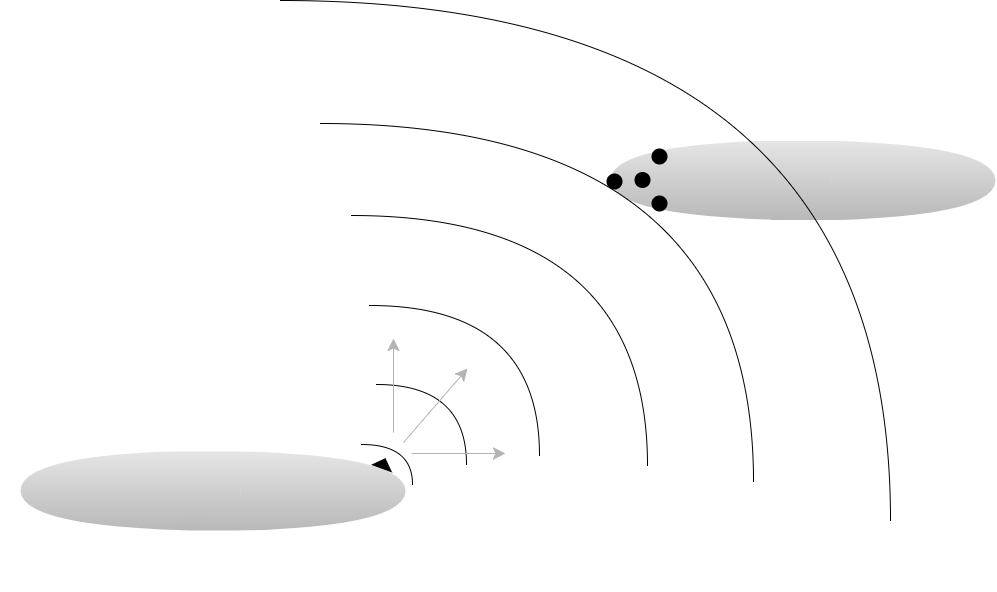
\includegraphics[width=0.6\textwidth]{figures/proposed-solution}
	\caption{Communication system}
	\label{fig:auv_scene}
\end{figure}

For a basic angle of arrival estimation in two dimensions between 2 hydrophones, A and B, as illustrated in figure \ref{fig:anglegeo}, the relationship between time delay and angle is given by equation \ref{eq:timeangle-2}. The \textit{c} is the speed of sound, \textit{$t_{A}$} and \textit{$t_{B}$} are the times of arrival of hydrophones A and B respectively, \textit{d} is the distance between the hydrophones and \textit{$\phi$} is the angle of arrival in respect to the direction of the baseline composed by A and B. 
\begin{eqnarray}
&c\ (t_{A} - t_{B})\ =\ dcos\phi
\label{eq:timeangle-2}
\end{eqnarray}
\begin{figure}[!htbp]
	\centering
	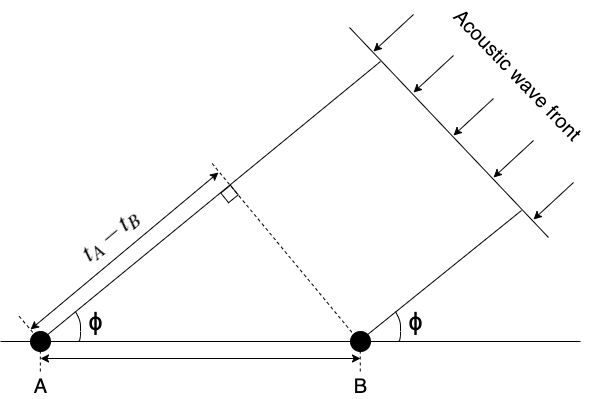
\includegraphics[width=0.7\textwidth]{figures/geohydro}
	\caption{2D angle of arrival estimation}
	\label{fig:anglegeo}
\end{figure}

Additionally, it is possible to calculate the range estimation as a mean all propagation times multiplied by the speed of sound \textit{c}, as in equation \ref{eq:range-estim}. \textit{N} is the number of hydrophones in the array and \textit{$t_{i}$} corresponds to time of arrival to each hydrophone.
\begin{eqnarray}
& R = c\ \frac{1}{N} \displaystyle\sum_{i=1}^{N} t_{i}
\label{eq:range-estim}
\end{eqnarray}

Since times are easily converted into distances, it is relatively easy to estimate the range of the communication. However, when calculating phase differences, there is no exact time notion, as it necessary to define a reference point. 

Considering sinusoidal signals, when having a array with four hydrophones spatially placed to form a 3D layout, the signal that is arriving to each  hydrophone in different times consequently have different phases. However, since sinusoidal signals are periodic, this means that for different signal periods the same phase value is observed, i.e. the phase is ambiguous. It is possible to observe this phenomenon in figure \ref{fig:phasediff}. In this illustration, $\alpha$ represents the observable phase difference of hydrophone H4 to the reference point H1. However, the actual phase difference which is intended to obtain, $\Delta$p4, is one period of the signal, $\lambda$, added to the observable phase $\alpha$.
\begin{figure}[!htbp]
	\centering
	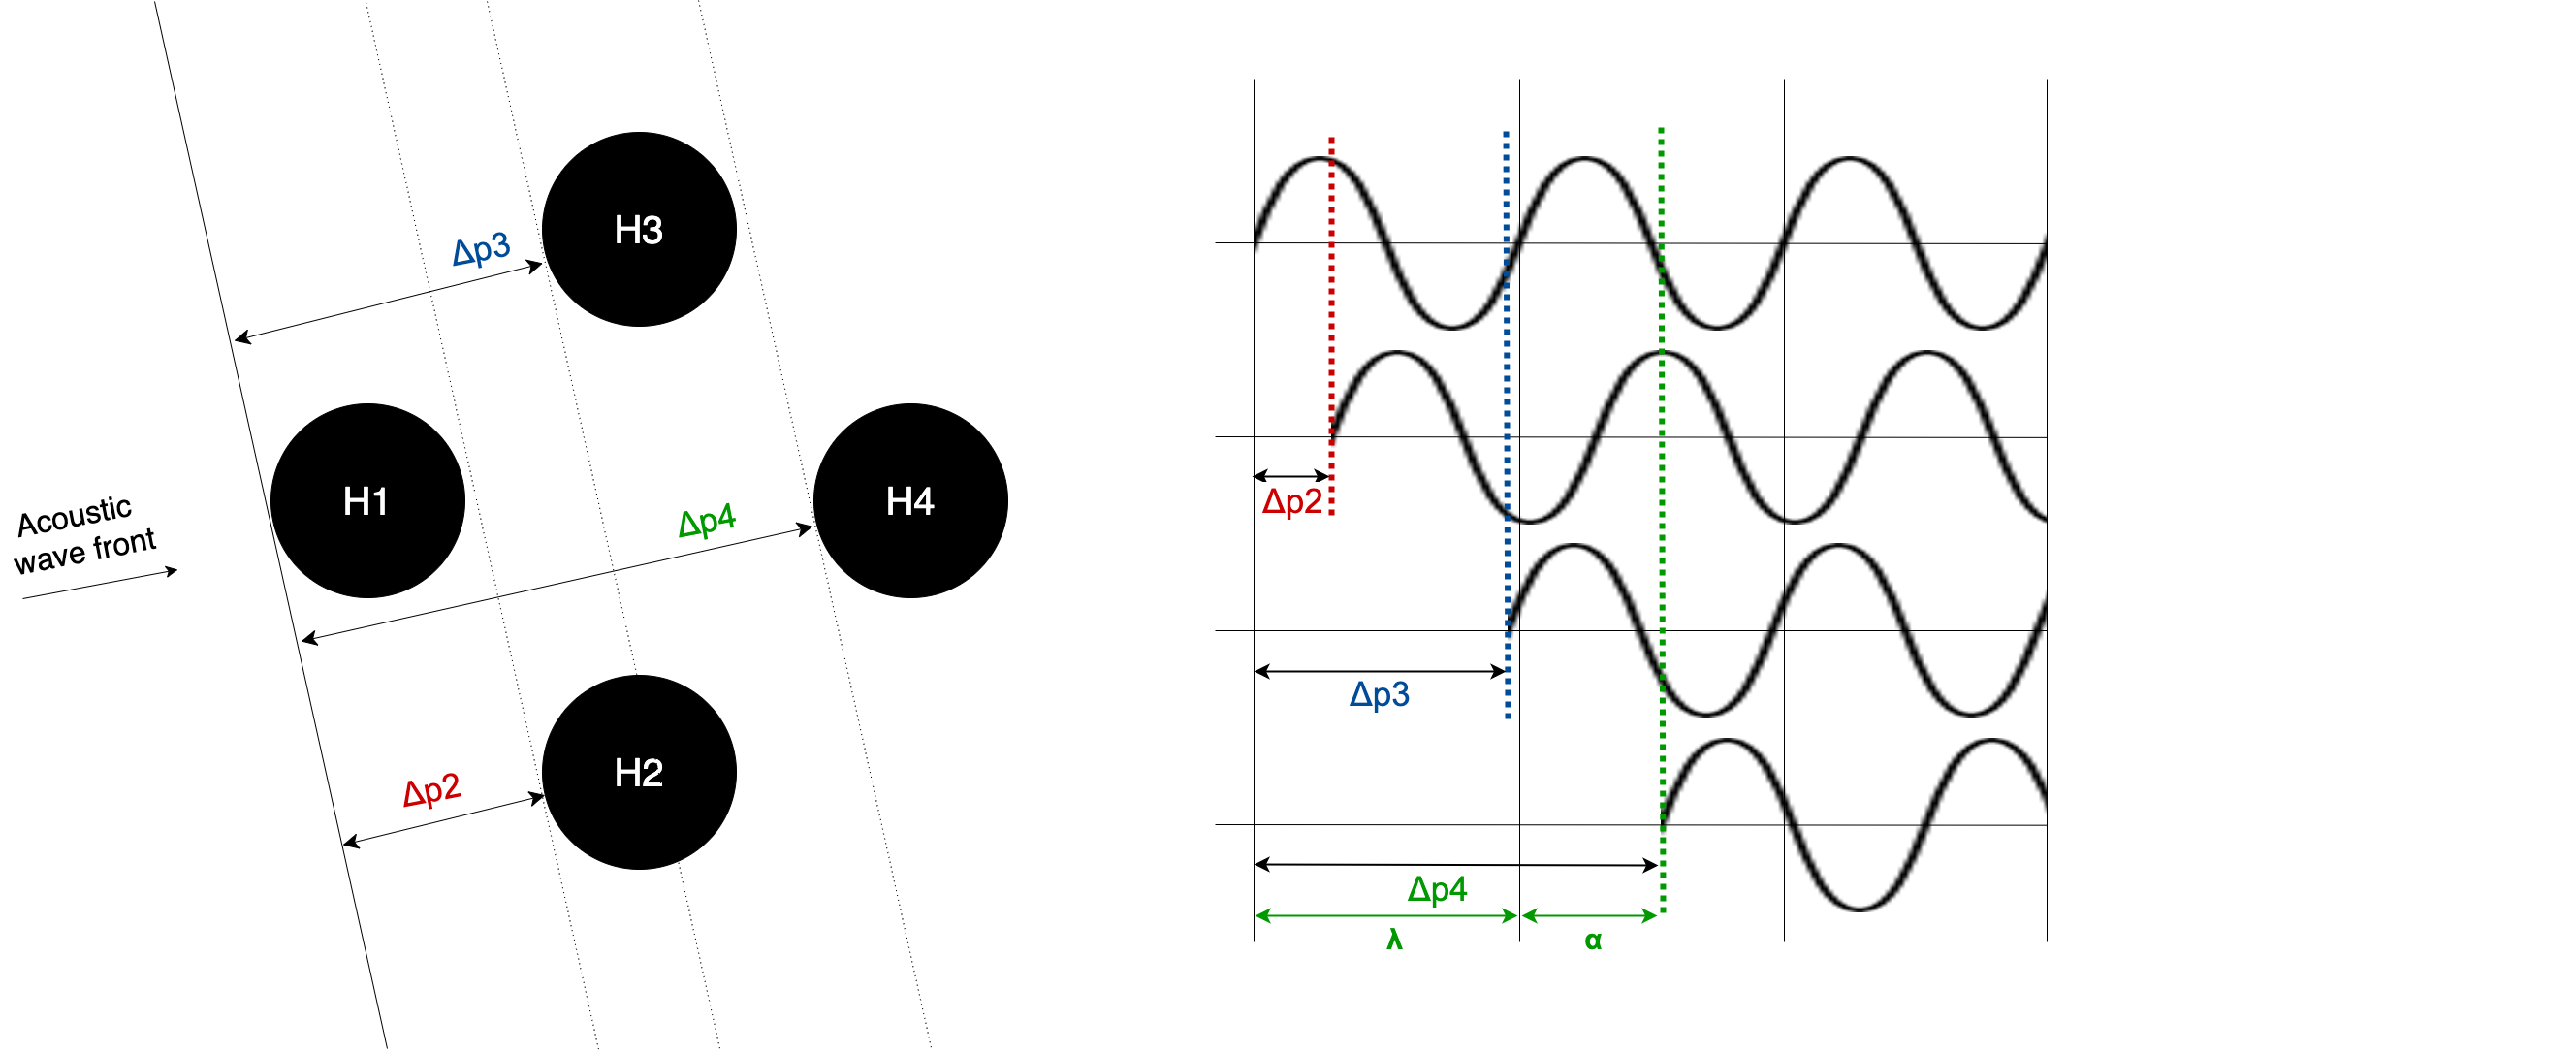
\includegraphics[width=1.2\textwidth]{figures/phase-diff}
	\caption{Phase difference to reference point and phase ambiguity}
	\label{fig:phasediff}
\end{figure}
For this reason, it is crucial to consider that the phase difference is given by the obtained phase value added by the number of periods ahead from the considered reference period.

In the system under study, the sent signals work with a operation frequency of 24.4 kHz. The corresponding signal period is $T = \frac{1}{24400} $ which, considering the underwater acoustic speed \textit{c} equal to 1500 m/s, the wavelength is approximately equal to $\lambda = \frac{T}{c} = 6.1 cm$. Having this into consideration, after obtaining the time of arrival of each hydrophone given by the cross correlation instances, besides the reference one, it is possible to conclude if the phase shift is superior to one period by analyzing if the time difference is greater than one period \textit{T}. In figure \ref{fig:phasediff}, each mentioned time difference between H1 and H2, H3 and H4 is converted to the corresponding phase differences $\Delta$p2, $\Delta$p3 and $\Delta$p4.

From this phase differences it is possible to estimate the angle from which the acoustic wave is coming from by comparing all pairs of hydrophones: H1-H2, H1-H3, H1-H4, H2-H3, H2-H4, H3-H4. 

One possibility to solve phase ambiguity in this system would be to place the four hydrophones with a baseline spacing inferior than $\frac{1}{2}$ of a wavelength. However, positioning the hydrophones closer together leads consequently to a increase on the estimation error. Additionally, since the hydrophones to be used in this system have a corresponding diameter of roughly half of a wavelength, they would not allow the mentioned configuration and so it will not be contemplated.
